\documentclass{standalone}
\usepackage{graphicx}	
\usepackage{amssymb, amsmath}
\usepackage{color}

\usepackage{tikz}
\usetikzlibrary{intersections, backgrounds}
\usepackage{pgfmath}

\definecolor{light}{RGB}{220, 188, 188}
\definecolor{mid}{RGB}{185, 124, 124}
\definecolor{dark}{RGB}{143, 39, 39}
\definecolor{highlight}{RGB}{180, 31, 180}
\definecolor{gray10}{gray}{0.1}
\definecolor{gray20}{gray}{0.2}
\definecolor{gray30}{gray}{0.3}
\definecolor{gray40}{gray}{0.4}
\definecolor{gray60}{gray}{0.6}
\definecolor{gray70}{gray}{0.7}
\definecolor{gray80}{gray}{0.8}
\definecolor{gray90}{gray}{0.9}
\definecolor{gray95}{gray}{0.95}

\begin{document}

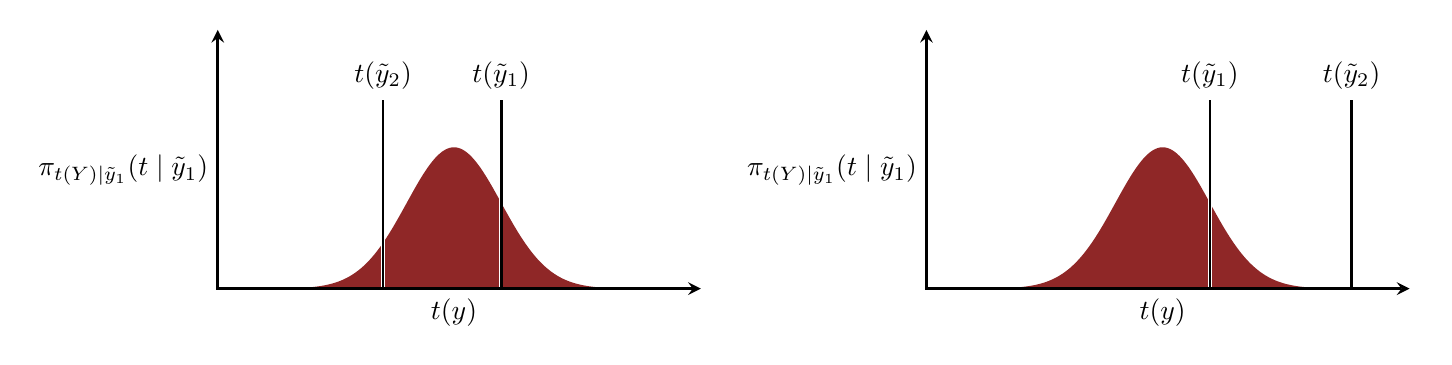
\begin{tikzpicture}[scale=0.3, thick,
declare function={ g(\x) = exp(-0.5 * (\x - 0) * (\x - 0) / (2 * 2)) / (2.506628274631001 * 2);}
]
  \pgfmathsetmacro{\dx}{0};
  \draw[color=white] (-18 + \dx, -2) rectangle (11 + \dx, 11);

  \fill[color=dark, domain=-10:10, smooth, samples=100, variable=\x] 
    plot ({\x + \dx}, {30 * g(\x)});

  \node[] at (-14 + \dx, 5) { $\pi_{t(Y) \mid \tilde{y}_{1}} (t \mid \tilde{y}_{1})$ };
  
  \draw [-, line width=1.5, color=white] (-3 + \dx, 0) -- (-3 + \dx, 8);
  \draw [-, line width=1, color=black] (-3 + \dx, 0) -- (-3 + \dx, 8)
  node [above] { $t(\tilde{y}_{2})$ };

  \draw [-, line width=1.5, color=white] (2 + \dx, 0) -- (2 + \dx, 8);
  \draw [-, line width=1, color=black] (2 + \dx, 0) -- (2 + \dx, 8)
  node [above] { $t(\tilde{y}_{1})$ };
  
  \draw [->, >=stealth, line width=1] (-10.05 + \dx, 0) -- +(20.5, 0);
  \draw [->, >=stealth, line width=1] (-10 + \dx, -0.05) -- +(0, 11);
  \node[] at (0 + \dx, -1) { $t(y)$ };


  \pgfmathsetmacro{\dx}{30};
  \draw[color=white] (-18 + \dx, -2) rectangle (11 + \dx, 11);

  \fill[color=dark, domain=-10:10, smooth, samples=100, variable=\x] 
    plot ({\x + \dx}, {30 * g(\x)});

  \node[] at (-14 + \dx, 5) { $\pi_{t(Y) \mid \tilde{y}_{1}} (t \mid \tilde{y}_{1})$ };
  
  \draw [-, line width=1.5, color=white] (8 + \dx, 0) -- (8 + \dx, 8);
  \draw [-, line width=1, color=black] (8 + \dx, 0) -- (8 + \dx, 8)
  node [above] { $t(\tilde{y}_{2})$ };

  \draw [-, line width=1.5, color=white] (2 + \dx, 0) -- (2 + \dx, 8);
  \draw [-, line width=1, color=black] (2 + \dx, 0) -- (2 + \dx, 8)
  node [above] { $t(\tilde{y}_{1})$ };
  
  \draw [->, >=stealth, line width=1] (-10.05 + \dx, 0) -- +(20.5, 0);
  \draw [->, >=stealth, line width=1] (-10 + \dx, -0.05) -- +(0, 11);
  \node[] at (0 + \dx, -1) { $t(y)$ };  
  
  
\end{tikzpicture}

\end{document}  